\chapter{Resultados}

Os testes foram feitos para comparar a taxa de entrega de pacotes, ao variar o método de envio utilizado POST ou PUT e a porcentagem de envio que simula a taxa de entrega de pacotes e o tempo de envio de cada mensagem, variando também o método utilizado e a porcentagem de envio. A variação da taxa de entrega foi de 10 a 100\%, variando de 10 em 10\% para cada amostra.

Objetivou-se, para o teste, a simulação da perda de pacotes, já que o foco do projeto é aplicar o código em sistemas embarcados com conexão sem fio.

Todos os testes foram feitos em dois computadores, conectados a redes sem fio, rodando o sistema operacional Linux, na distribuição Linux Mint, que visa a simular um servidor para receber os dados e o cliente embarcado que faz o envio da mensagem.

\section{PUT}

A figura \ref{fig:put_tempo_envio} mostra o primeiro teste, para comparação posterior, do tempo de envio de mensagens do tipo PUT.

\begin{figure}[!htb]
	\centering
	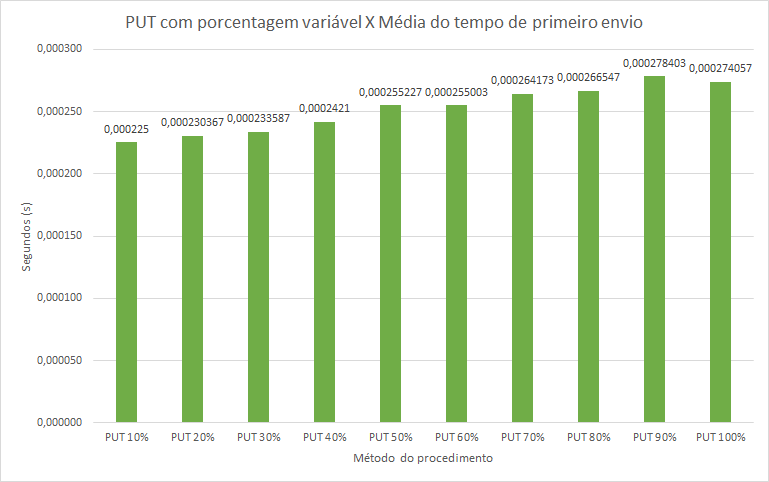
\includegraphics[width=.8\textwidth]{../imagens/PUTxPrimeiroEnvio}
	\caption{Tempo de envio}
	\label{fig:put_tempo_envio}
\end{figure}

\section{POST 1 tentativa}
No primeiro teste, conforme a figura \ref{fig:put_num_entregues},
será demonstrado o número de mensagens entregues, usando o tipo de mensagem POST, com taxa de erro de pacote de 10 a 100\%.
Esse teste simulará a taxa de entrega de um método PUT.

\begin{figure}[!htb]
	\centering
	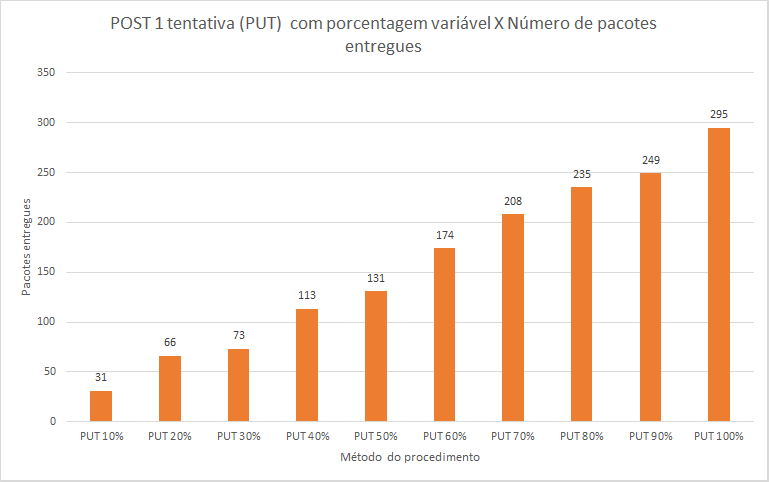
\includegraphics[width=.8\textwidth]{../imagens/PUTxNumentregues}
	\caption{Número de mensagens entregues}
	\label{fig:put_num_entregues}
\end{figure}

Como esperado, existe um ganho considerável de pacotes entregues, ao aumentar o parâmetro de porcentagem de entrega, variando praticamente na mesma proporção de pacotes entregues com a porcentagem definida no código.

\section{POST 5 tentativas}

O primeiro teste deste método, conforme figura \ref{fig:post_num_entregues}, mostra o número de mensagens do tipo POST entregues, segundo a variação da porcentagem de envio entre 10 a 100\%.
É importante lembrar que uma mensagem do tipo POST faz cinco tentativas de envio da mensagem.

\begin{figure}[!htb]
	\centering
	\includegraphics[width=0.8\textwidth]{../imagens/POSTxNumEntregues}
	\caption{Número de mensagens entregues}
	\label{fig:post_num_entregues}
\end{figure}
\hfill \break
\hfill \break
\hfill \break
\hfill \break
\hfill \break

O segundo teste será o tempo de envio da primeira mensagem, para o método POST.

\begin{figure}[!htb]
	\centering
	\includegraphics[width=.8\textwidth]{../imagens/POSTxPrimeiroEnvio}
	\caption{Tempo de envio}
	\label{fig:post_tempo_envio}
\end{figure}

E por último, expõe-se o gráfico da média do tempo de recebimento do ACK para o método POST, na figura \ref{fig:post_media_tempo_ACK}.

\begin{figure}[!htb]
	\centering
	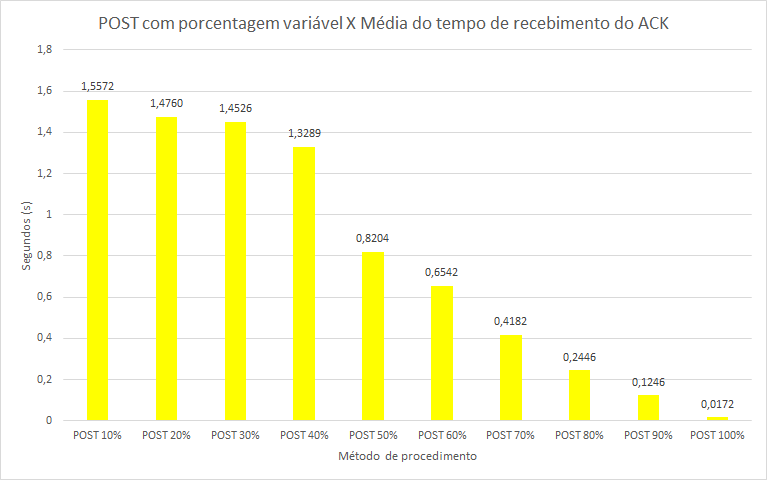
\includegraphics[width=.8\textwidth]{../imagens/POSTxMediatempopacoteentregue}
	\caption{Tempo de envio}
	\label{fig:post_media_tempo_ACK}
\end{figure}

\hfill \break
\hfill \break
\hfill \break

\section{Comparação de resultados}

Agora, passa-se às comparações dos métodos PUT e POST com uma tentativa, e POST com cinco tentativas.
A primeira comparação, feita na figura \ref{fig:num_entregues_post5_post1}, é entre o método POST com cinco tentativas e o método PUT, em relação ao número de mensagens entregues.

\begin{figure}[!htb]
	\centering
	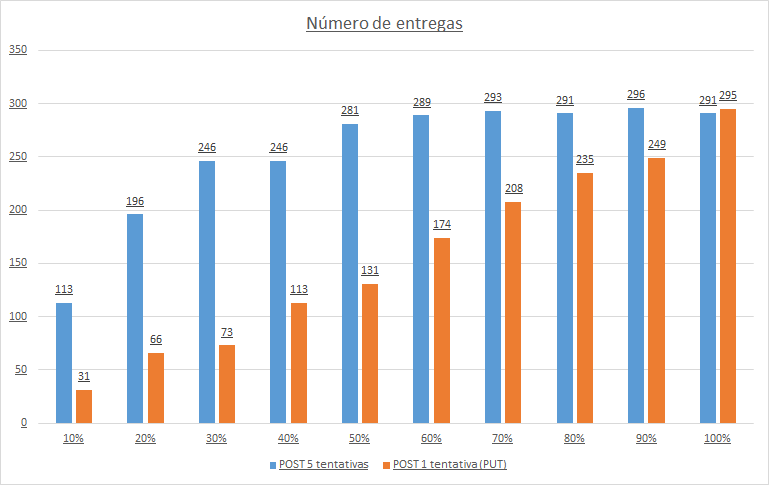
\includegraphics[width=.8\textwidth]{../imagens/Numero_entregas_PUTxPOST}
	\caption{Número de mensagens entregues}
	\label{fig:num_entregues_post5_post1}
\end{figure}

Como é observado, o número de mensagens entregues com cinco tentativas de entrega é muito superior em quase todos os testes; eles apenas se igualam quando a chance de entrega chega a 100\%. Isso comprova que, se a confiabilidade na entrega for fator importante, o aumento de tentativas de entrega é algo a se levar em conta. Em casos em que a taxa de entrega seja ainda inferior, é possível aumentar o número de tentativas de entrega para maior segurança.

Então, na figura \ref{fig:tempo_envio_1_msg_post5_put}, observa-se a comparação entre os métodos PUT e POST, para comparar o tempo gasto para envio da mensagem.

\begin{figure}[!htb]
	\centering
	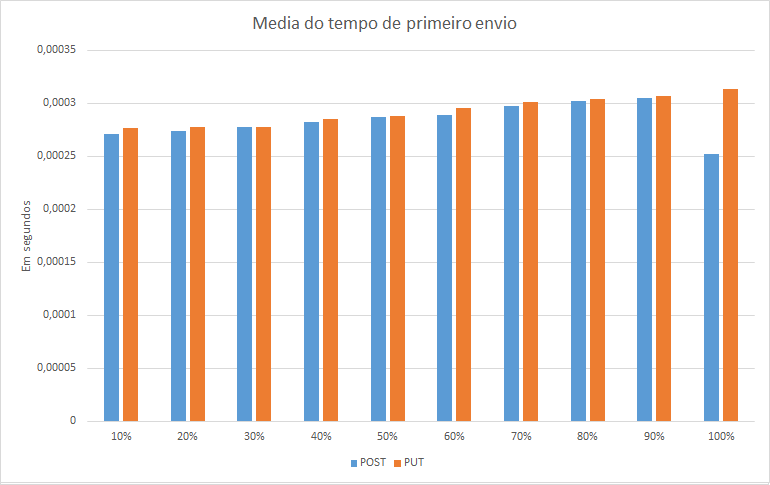
\includegraphics[width=.8\textwidth]{../imagens/media_primeiro_envio_PUTxPOST}
	\caption{Tempo de envio  da primeira mensagem}
	\label{fig:tempo_envio_1_msg_post5_put}
\end{figure}

Aqui é possível verificar a eficiência do método PUT, afinal, o tempo de execução é em média 10\% menor, já que este não precisa armazenar o dado enviado, pois é finalizado após o envio do programa, ao contrário do método POST, que ainda executa a função \texttt{buffer\_msg}, para achar uma posição em buffer e salvar a mensagem. Este método pode ser escolhido no caso de a perda de pacotes não ser tão relevante, ou, então, quando a taxa de entrega chegar próxima a 100\%.


